\section{Aufgabe 1}
Im Rahmen dieser Aufgabe soll die Schallgeschwindigkeit in Luft direkt gemessen werden. Indem die Zeit gemessen wird, die ein Signal braucht um eine gewisse Strecke zurückzulegen.
\subsection{Aufbau}
Der Versuchsaufbau besteht aus einer Klatsche, die bei Betätigung einen akustischen Impuls abgibt. Um die Zeit zu messen, die das Signal bis zu einem bestimmten Punkt benötigt wird bei der Betätigung der Klatsche zusätzlich ein elektronisches Signal abgeben, dieses wird vom Oszilloskop als \textit{Trigger} benutzt. An dem Ende der Messstrecke wird ein Mikrophon aufgebaut, dass an das Oszilloskop angeschlossen wird. Auf dem Oszilloskop kann dann die Zeit zwischen dem Triggersignal und einem Ausschlag durch den vom Mikrophon aufgenommen Schall bestimmt werden. Verwendet wird ein Digitales Oszilloskop, dass die Daten direkt an den Computer überträgt, damit sie gut gespeichert werden können.
\subsection{Fehlerabschätzung}
Der Fehler der Messung setzt sich aus einer Ungenauigkeit der Streckenmessung und einem Fehler der Zeitmessung zusammen.

Bei der Streckenmessung kommt zu den Messungenauigkeiten noch ein systematischer Fehler, da nicht absehbar ist, wo sich das Mikrophon genau in der Apparatur befindet, außerdem ist auch nicht klar, was als Ausgangspunkt des akustischen Signals gelten soll. Um das in der Rechnung zu berücksichtigen wird \(s\) mit einem systematischen Fehler \(s_{sys}\) addiert.

Auch bei der Messung der Zeit ist ein systematische Fehler vorhanden dessen Ursache nicht genau klar ist, da kaum etwas über die Geräte bekannt ist. Eine Mögliche Ursache ist, dass eventuell das Trigger- oder das akustische Signal nicht Verzögerungsfrei weitergeleitet wird. Daher wird auch hier ein \(t_{sys}\) addiert.
\begin{align}
s_{mess} &= s + s_{sys}\\
t_{mess} &= t + t_{sys}
\end{align}

Die statistischen sind schwer abzuschätzen. Es ist unter Anderem nicht immer klar ist, wann genau das akustische Signal detektiert wurde. Ein Fehlerwert dennoch nur schätzbar, daher werden im Anschluss die Fehler aus der Streuung herangezogen.

\subsection{Messwerte}
Eine Messung lieferte zu jeder gewählten Distanz eine v-t-Kurve, in der die Zeit zwischen Triggersignal und akustischem Signal abgelesen werden kann. Die Werte sind dabei nur mit dem Auge ermittelt worden. Um sich das besser vorstellen hier eine Beispielkurve:

\begin{center}
\begin{minipage}{\linewidth}
\centering
\makebox[0cm]{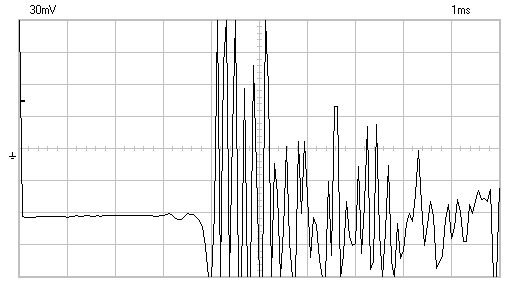
\includegraphics[width=\textwidth]{graphen/a1/100_1.png}}
\captionof{figure}{Beispielhafte Ausgabe des Digitaloszilloskops bei s = 1m}
\end{minipage}
\label{bsp}
\end{center}
Die Zeit wurde bei diesem Beispiel geschätzt auf \(t = 3,9\, ms\). Bei den weiteren Messungen wurde identisch verfahren.
%Aufgenommen wurden zwei Messreihen, deswegen sind zu jeder Strecke zwei Zeitmessungen vorhanden.
Zusammengefasst wurden folgende Werte ermittelt:
\begin{center}
\begin{tabular}{c|c}
Strecke \(s\) in \(cm\) & Zeit \(t\) in \(ms\) \\\hline
\(100\) & \( 3.9\) \\
\(100\) & \( 4\) \\
\(110\) & \( 4.1\) \\
\(110\) & \( 4.1\) \\
\(120\) & \( 4.7\) \\
\(120\) & \( 4.5\) \\
\(130\) & \( 4.8\) \\
\(130\) & \( 5.1\) \\
\(140\) & \( 4.9\) \\
\(140\) & \( 5.1\) \\
\(150\) & \( 5.2\) \\
\(150\) & \( 5.4\) \\
\(160\) & \( 5.5\) \\
\(160\) & \( 5.7\) \\
\(170\) & \( 5.8\) \\
\(170\) & \( 5.9\) \\
\(180\) & \( 5.9\) \\
\(180\) & \( 6\) \\
\(190\) & \( 6.7\) \\
\(190\) & \( 6.1\) \\
\end{tabular}
\captionof{table}{Abgelesene Zeiten für verschiedene Strecken}
\end{center}
\subsection{Graphen}
Um diese Messwerte auszuwerten werden sie zunächst in ein s-t-Diagramm eingetragen und anschließend eine Ausgleichsgerade mit einem Fehler aus der Streuung eingefügt:
\begin{center}
\begin{minipage}{\linewidth}
\centering
\makebox[0cm]{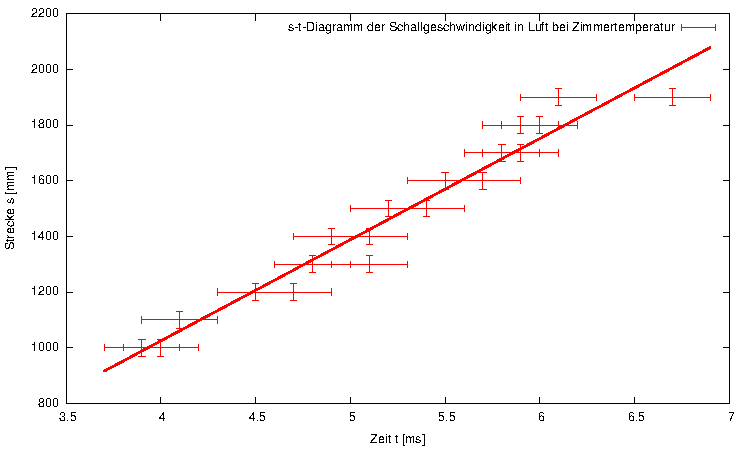
\includegraphics[width=\textwidth]{graphen/gnuplot/a1}}
\captionof{figure}{Beispielhafte Ausgabe des Digitaloszilloskops bei s = 1m}
\end{minipage}
\label{bsp}
\end{center}
Um die Plausibilität der Ausgleichsgeraden zu überprüfen wurden die Fehler geschätzt:
\begin{align}
\Delta t & = 30\, ms \notag \\
\Delta s & = 2\, cm \notag
\end{align}
Die lineare Regression wurde mit einer Funktion \(s(t) = a + b \cdot t\) durchgeführt und ergab folgende Parameter:
\begin{align}
a &= \left(-430 \pm 93 \right)\, mm \notag \\
b &= \left( 363 \pm 18 \right)\, \frac{m}{s} \notag
\end{align}
\subsection{Auswertung}
Die Geschwindigkeit ist allgemein definiert als:
\begin{align}
v = \frac{ds}{dt}
\end{align}
angewendet auf die Funktion der linearen Regression ergibt für die Schallgeschwindigkeit:
\begin{align}
c &= \frac{d}{dt} \left(a + b \cdot \left(t - t_{sys} \right) - s_{sys} \right) \label{drv}\\
\Rightarrow c &= b \\
\Rightarrow c &= \left( 363 \pm 18 \right)\, \frac{m}{s} \notag
\end{align}
\subsection{Fazit und Vergleich}
Der Versuch war sehr gut durchführbar, die Streuung der Messwerte ist zwar recht groß, jedoch ist zu sehen, dass alle Messwerte mit den geschätzten Fehlern die Ausgleichsgerade schneiden. Die ermittelte Schallgeschwindigkeit ist:
\begin{align}
c = \left( 360 \pm 20 \right)\, \frac{m}{s} \notag
\end{align}
Dieses Ergebnis ist identisch zum Literaturwert, dieser liegt bei Zimmertemperatur bei ca. \(343\, \frac{m}{s}\).

Interessant ist, dass der systematische Fehler \(a\) mit ca. \(-43\, cm\) extrem groß ist. Der Grund dafür, kann nur sein, dass auch \(t\) einen signifikanten systematischen Fehler enthält da die Strecke nicht so ungenau gemessen wurde. Da \(a\) negativ ist muss also auch \(t_{sys}\) negativ sein. Das kann nur heißen, dass das Triggersignal zu spät übermittelt wird.

